Generative adversarial network (GAN) is a well-known machine learning model proposed by Goodfellow. It has outstanding performance in various challenging tasks, especially in image generation and video generation tasks. The general GAN consists of a generator ${G}$ and a discriminator ${D}$. It accomplishes generation tasks through an adversarial game of ${G}$ and ${D}$. During the training, ${G}$ is trained to maximize the probability that ${D}$ misclassifies the generated data as the real data. Correspondingly, ${D}$ is trained to maximize the probability of successfully classifying real data, while minimizing the probability of misclassifying generated data. The optimization of GAN can be summarized as
\begin{equation}
  \begin{split}
    \mathop {\min }\limits_G \mathop {\max }\limits_D V(D,G) = {\rm{ }}{{\rm{E}}_{x\sim{p_r}(x)}}[\log D(x)]
    \\+ {{\rm{E}}_{z\sim{p_z}(z)}}[\log (1 - D(G(z)))]. \label{eq1}
  \end{split}
\end{equation}

QGAN, as a quantum version of GAN, has more advantages in sampling and generating discrete data than its classical counterpart. In addition, it has been proved the potential exponential speedup theoretically~\cite{lloyd2018quantum}. These lead to extensive research on QGAN. For example, the learning of the classical or quantum data~\cite{benedetti2019adversarial, zeng2019learning, zoufal2019quantum,ahmed2021quantum}, using the entangling power of quantum circuits to overcome issues of non-convexity and mode collapse~\cite{niu2022entangling}, discovering small molecular drugs~\cite{li2021quantum}, data enhancement~\cite{nakaji2021quantum} and anomaly detection with QGAN~\cite{herr2021anomaly}.

We show an example of using mindquantum, building a hybrid quantum-classical generative adversarial network(QC-GAN), and then learning a probability distribution to generate handwritten digits through training. Specifically, the QC-GAN consists of a variational quantum circuit with one layer of neural network to form ${G}$ and a classical neural network to form ${D}$. It is trained similarly to the classical GAN with a noise vector input ${z}$ to the ${G}$. Then, the adversarial training of ${G}$ and ${D}$ realizes the generation of images
Differently, the generated image is obtained by quantum circuit evolution, measurement, and nonlinear mapping of the neural network. The overall structure and training process of QC-GAN is shown in Fig~\ref{qc-gan}.

\begin{figure}[ht]
  \centering
  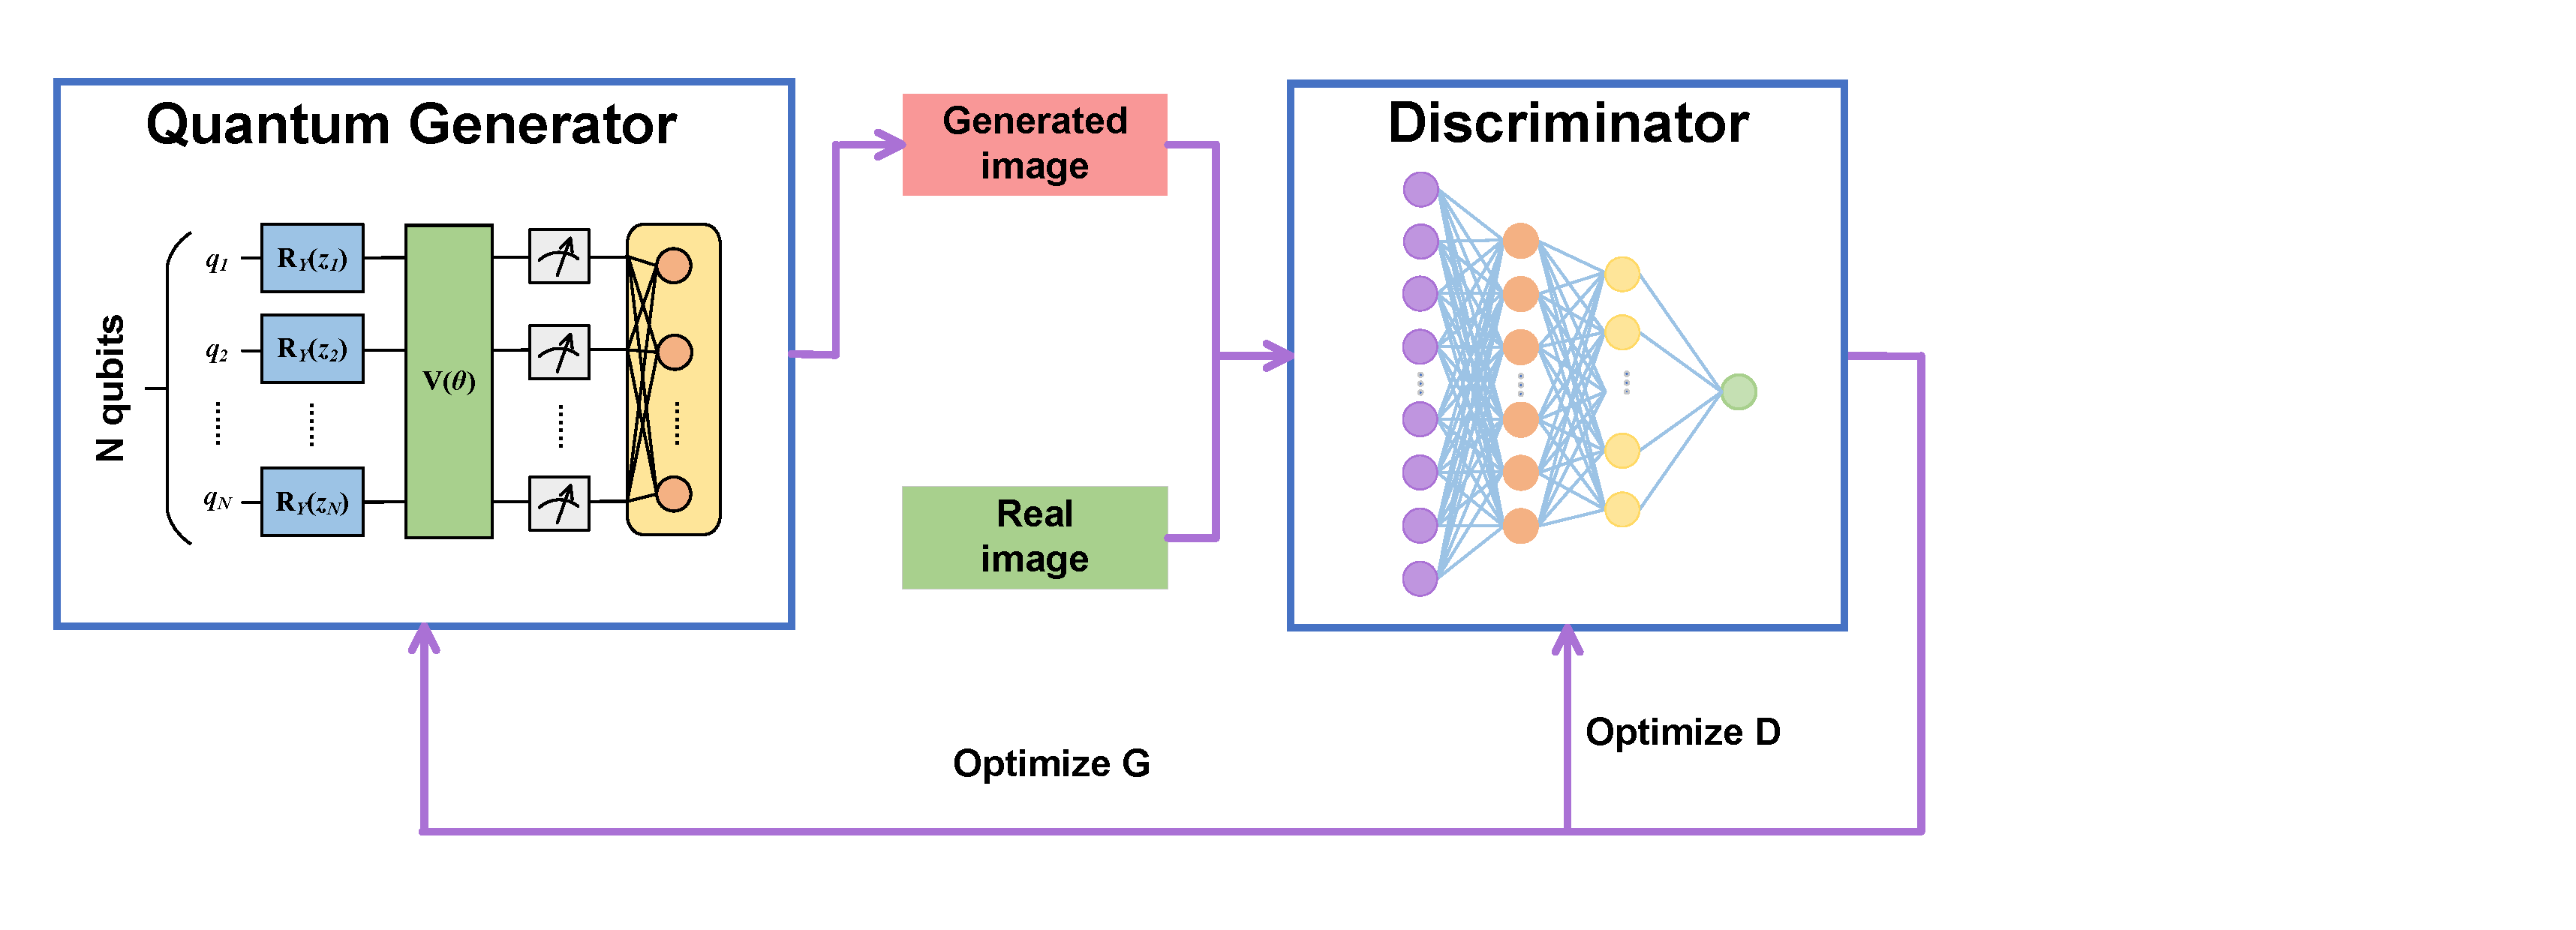
\includegraphics[scale=0.2]{qc-gan.pdf}
  \caption{\label{qc-gan} The overall architecture and training process of QC-GAN.}
\end{figure}

The first step is loading the dataset. The experiment uses the handwritten digit set, which has a total of 70,000 handwritten digit images, including 60,000 training samples and 10,000 test samples, with an image size of 28*28 and a single channel. After loading the dataset, a series of preprocessing operations are also performed to prepare for subsequent training. The model build-up consists of two networks, the generator ${G}$ and the discriminator ${D}$. For the discriminator part, it uses a general fully connected network structure. For the generator, it is divided into two parts, the quantum part and the classical part. Quantum circuits are built by calling the parameterized rotation gates of MindQuantum. The quantum circuit is constructed as follows.The structure of the quantum circuit can be shown through ${circuit.summary}$.
\begin{figure*}[htbp]
  \centering
  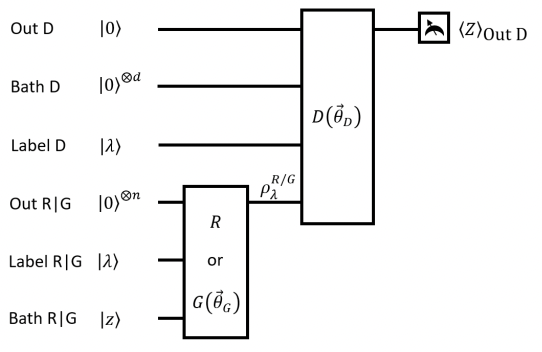
\includegraphics[scale=0.5]{circuit}
  \caption{\label{quantum-circuit} The quantum circuit.}
\end{figure*}

\begin{lstlisting}
  def quantum_circuit():
    encoder = Circuit()
    for i in range(qubits):
        encoder += RY(f'noise{i}').on(i)
    encoder = encoder.no_grad()
    ansatz = Circuit()
    for i in range(depth):
        for k in range(gate):
            for j in range(qubits):
                if k == 0:
                    ansatz += RX(f'weights{i}{j}{k}').on(j)
                elif k == 1:
                    ansatz += RZ(f'weights{i}{j}{k}').on(j)
                elif k == 2:
                    if j < 4:
                        ansatz += RX(f'weights{i}{j}{k}').on(j + 1, j)
                    else:
                        ansatz += RX(f'weights{i}{j}{k}').on(0, j)
    circuit = encoder.as_encoder() + ansatz.as_ansatz()
    return circuit
\end{lstlisting}
Stacking quantum circuits in layers and measuring the outputs constitutes a quantum layer.
\begin{lstlisting}
def quantum_layer(qubits):
    circuit = quantum_circuit()
    circ_l = Circuit()
    hams = quantum_measure(qubits)
    sim = Simulator('mqvector', circuit.n_qubits)
    sim_l = Simulator('mqvector', qubits)
    grad_ops = sim.get_expectation_with_grad(hams, circuit, circ_l, sim_l, parallel_worker=4)

    QuantumNet = MQLayer(grad_ops,
                         weight=ms.Tensor(np.random.uniform(-np.pi, np.pi, len(circuit.ansatz_params_name)),
                         dtype=ms.dtype.float32))
    return QuantumNet
\end{lstlisting}

Then, similar to the classical neural network construction, each layer of the network is defined and the forward propagation process is set to constitute the quantum generator model. The backward process automatically derives and updates the parameters.
\begin{lstlisting}
  class QuantumGenerator(nn.Cell):
    def __init__(self):
        super(QuantumGenerator, self).__init__()
        self.quantumlayer = quantum_layer(qubits)
        self.linear = nn.Dense(2**qubits, img_size * img_size, weight_init='uniform')
        self.relu = nn.ReLU()
        self.sigmoid = nn.Sigmoid()
        self.tanh = nn.Tanh()

    def construct(self, x):
        x = self.quantumlayer(x)
        x = x/(abs(x).max())
        x = self.linear(x)
        out = self.sigmoid(x)
        return out
\end{lstlisting}

The parameters of the quantum circuits are optimized according to the designed cost function. The generator needs to generate a probability distribution as real as possible, and the discriminator needs to distinguish between the real distribution and the generated distribution as much as possible. Their cost functions are designed separately as follow.
\begin{equation}
  {L_G} =  - {{\rm E}_{x\sim{p_f}(x)}}\left[ {\log D(x)} \right],
\end{equation}
\begin{equation}
  {L_D} =  - {{\rm E}_{x\sim{p_r}(x)}}\left[ {\log D(x)} \right] - {{\rm E}_{x\sim{p_f}(x)}}\left[ {\log D(x)} \right].
\end{equation}

According to the designed loss function and model, the generator and discriminator are trained and parameters are updated in turn.After training, the noise vector is used as input to the generator and the generated handwritten digits are output and the results are shown in Fig~\ref{qgan-result}. It can be seen that as the number of iterations increases, the input noise is gradually able to produce a clear digital image. Notably, the number of iterations for training needs to be carefully designed and not more is better.
\begin{figure}[htbp]
  \centering
  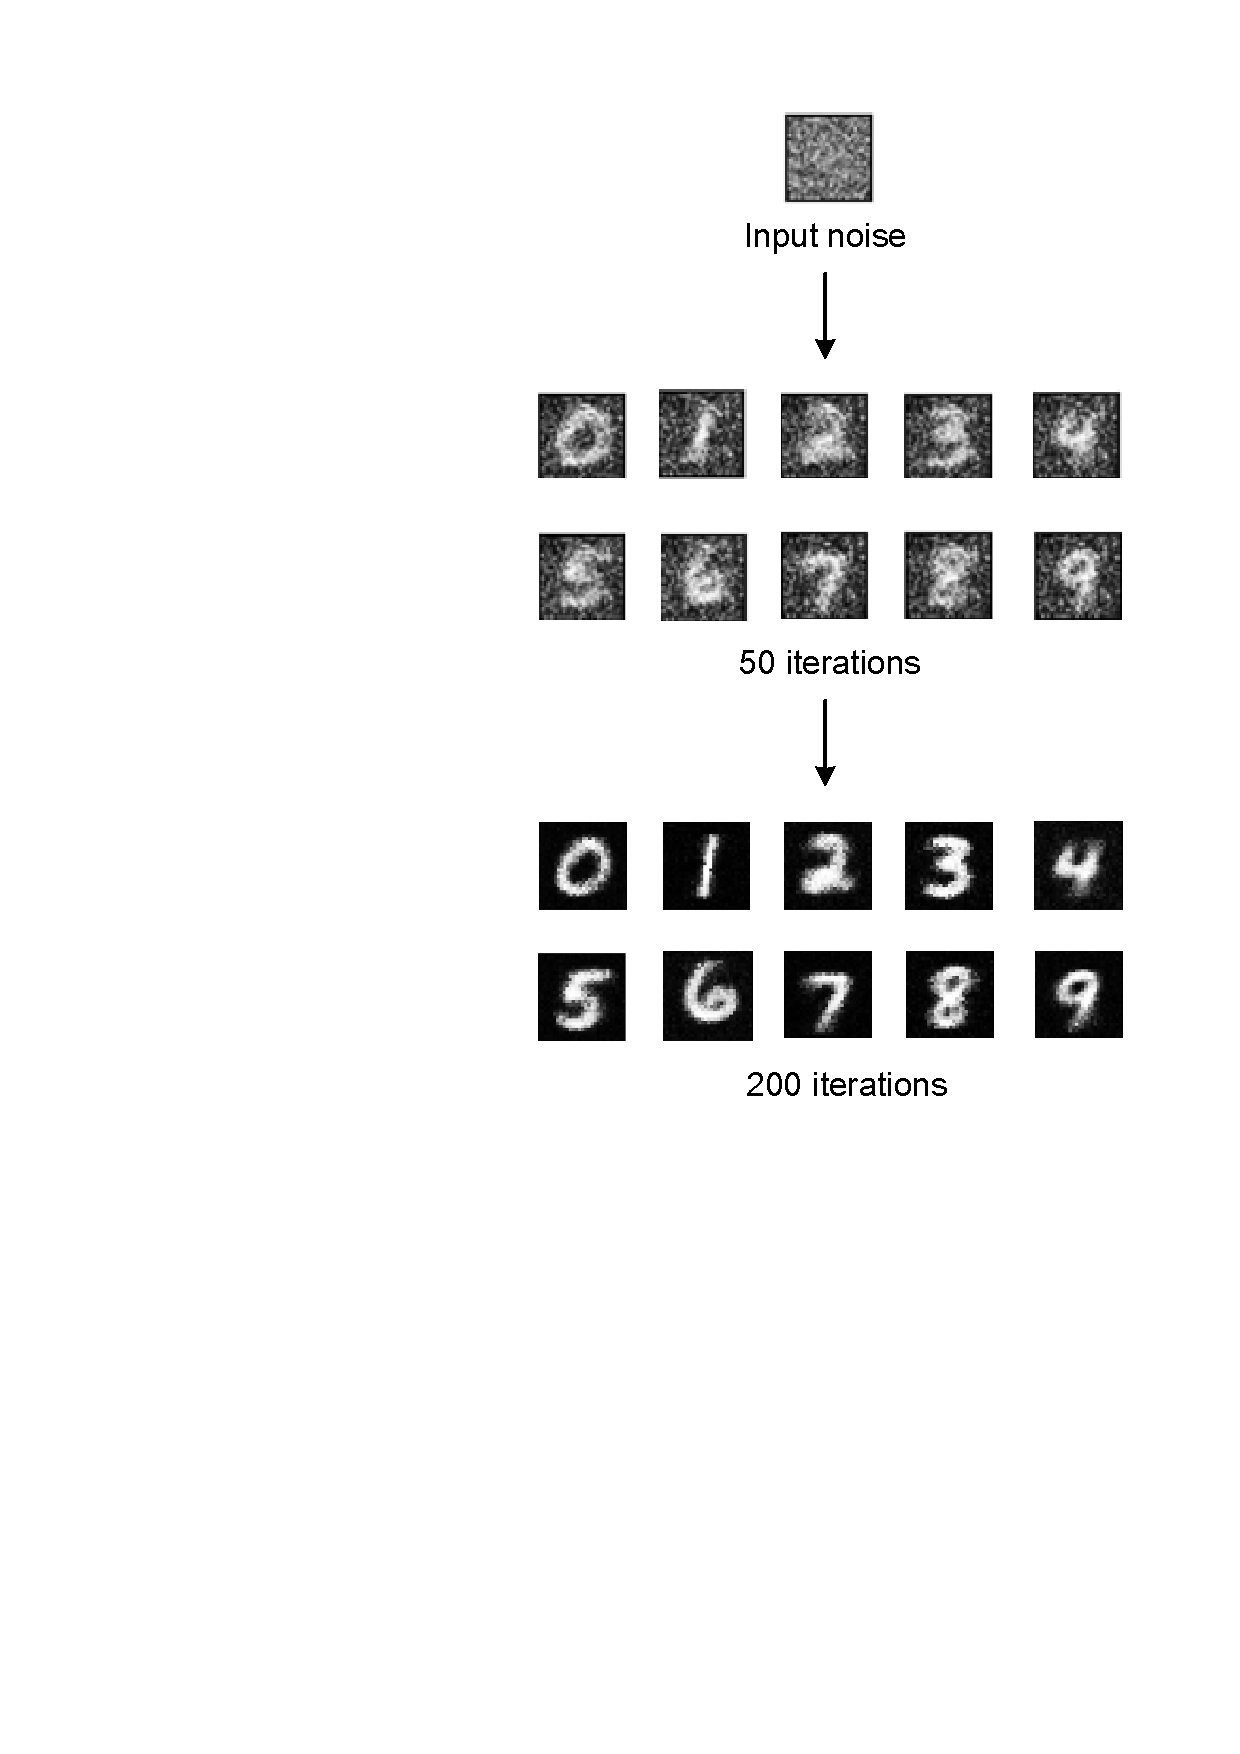
\includegraphics[scale=0.5]{qgan-result.pdf}
  \caption{\label{qgan-result} The algorithms based on PQCs are optimized in classical and quantum systems.}
\end{figure}